\chapter{二阶差分扩频通信系统原理}
\section{直接序列扩频的基本原理}
信道无差错传输信息的最大信息速率为信道容量\citeup{文元美2005现代通信原理},记为$C$。根据香农公式,加性高斯白噪声功率为$N$,信道的带宽为$B$,信号功率为$S$的连续信道的的信道容量$C$为
\begin{equation}
C=B\log_2\left[1+\frac{S}{N}\right]
\end{equation}
在信道容量$C$一定时,为了降低$S/N$(信噪比)的要求,可以增大带宽$B$。换言之,在信噪比无法提高时可以通过增大带宽来提高信道容量。直接序列扩频正是增大带宽,以减小系统对信噪比$S/N$的要求。
\subsection{直接序列扩频过程}
图\ref{fig:ddcode:dsss}中$a(t)$为原始数据码元,$c(t)$为扩展频谱的码元,$d(t)$为传输的基带信号。为了能够将$a(t)$的频谱展宽,将$a(t)$与一个频谱比自己宽很多的$c(t)$相乘得到$d(t)$。$d(t)$的频谱宽度与$c(t)$相当,图\ref{fig:ddcode:dsss}中的频谱只是示意,实际$d(t)$的频谱要复杂得多。

\begin{figure}[htbp]
	\centering
	\def \nod{~~~~}
\def \zihao{\wuhao}
	\tikzstyle{neuron}=[circle,fill=black!25,minimum size=0pt,inner sep=0pt]
	\tikzstyle{num}=[circle,fill=red!25,minimum size=0pt,inner sep=0pt]

\begin{tikzpicture}[>=stealth',node distance=2cm]
	\def\intevel{0.25cm} %码宽度
	\def\hl{0.8cm}
	\def\gl{4}

	%% a(t)
	\path[draw] (0,0)
		--++(\gl*\intevel,0)
		--++(0,\hl)
		--++(2*\gl*\intevel,0)
		--++(0,-\hl)
		--++(\gl*\intevel,0)
		--++(0,\hl)
		--++(\gl*\intevel,0)
		;
	\draw
		(3cm,1cm) --++(0,0.5cm)
		(4cm,1cm) --++(0,0.5cm);
	\draw node[name=mrk1] at(3.5cm,1.25cm) {\small$T_s$};
	\draw [->] (mrk1)--(3cm,1.25cm);
	\draw [->] (mrk1)--(4cm,1.25cm);
	\draw node[xshift=-0.5cm,yshift=.4cm] at(0,0) {$a(t)$};
	\coordinate (o1) at (6cm,0);
	\coordinate (o2) at (10cm,0);
	\draw[->] (o1)--(o2) node[right]{$f$};
	\draw[->] (8cm,-0.2cm) --+(0,1.4cm) node[left] {\xiaowu 幅度};
	\draw[xshift=8cm,thick] plot[samples=300,domain=-1.5:1.5,id=x2] function{sin(80*x)/(80*x)};
	
	% c(t)
	\draw (0,-1.5cm+\hl)
		--++(2*\intevel,0)
		--++(0,-\hl)
		--++(\intevel,0)
		--++(0,\hl)
		--++(\intevel,0)
		--++(2*\intevel,0)
		--++(0,-\hl)
		--++(\intevel,0)
		--++(0,\hl)
		--++(\intevel,0)
		--++(2*\intevel,0)
		--++(0,-\hl)
		--++(\intevel,0)
		--++(0,\hl)
		--++(\intevel,0)
		--++(2*\intevel,0)
		--++(0,-\hl)
		--++(\intevel,0)
		--++(0,\hl)
		--++(\intevel,0)
		--++(2*\intevel,0)
		--++(0,-\hl)
		--++(\intevel,0)
		--++(0,\hl)
		--++(\intevel,0)
		;
	\draw node at(2.7cm,-0.5cm) {\small$T_c$};
	
	\draw node[xshift=-0.5cm,yshift=.4cm] at(0,-1.5cm) {$c(t)$};
	\coordinate (o1) at (6cm,-1.5cm);
	\coordinate (o2) at (10cm,-1.5cm);
	\draw[->] (o1)--(o2) node[right]{$f$};
	\draw[->] (8cm,-1.7cm) --+(0,1.4cm) node[left] {\xiaowu 幅度};
	\draw[xshift=8cm,yshift=-1.5cm,thick] plot[samples=300,domain=-1.5:1.5,id=x3] function{sin(5*x)/(5*x)};
	
	% d(t)
	\draw (0,-3cm)
	--++(2*\intevel,0)
	--++(0,\hl)
	--++(\intevel,0)
	--++(0,-\hl)
	--++(\intevel,0)
	--++(0,\hl)
	--++(2*\intevel,0)
	--++(0,-\hl)
	--++(\intevel,0)
	--++(0,\hl)
	--++(\intevel,0)
	--++(2*\intevel,0)
	--++(0,-\hl)
	--++(\intevel,0)
	--++(0,\hl)
	--++(\intevel,0)
	--++(0,-\hl)
	--++(2*\intevel,0)
	--++(0,\hl)
	--++(\intevel,0)
	--++(0,-\hl)
	--++(\intevel,0)
	--++(2*\intevel,0)
	--++(0,\hl)
	--++(\intevel,0)
	--++(0,-\hl)
	--++(\intevel,0)
	;
	\draw node[xshift=-0.5cm,yshift=.4cm] at(0,-3cm) {$d(t)$};
	\coordinate (o1) at (6cm,-3cm);
	\coordinate (o2) at (10cm,-3cm);
	\draw[->] (o1)--(o2) node[right]{$f$};
	\draw[->] (8cm,-3.2cm) --+(0,1.4cm) node[left] {\xiaowu 幅度};
	\draw[xshift=8cm,yshift=-3cm,thick] plot[samples=300,domain=-1.5:1.5,id=x3] function{sin(5*x)/(5*x)};
	
	% label 
	\draw node at (2.2cm,-3.8cm) {\wuhao 码元波形};
	\draw node at (8cm,-3.8cm) {\wuhao 码元频谱};
	
\end{tikzpicture}
	\caption{直接序列扩频示意图}
	\label{fig:ddcode:dsss}
\end{figure}

$c(t)$由伪随机码(Pseudo Code)$c[n]$产生,伪随机码具有一下特性:
\begin{hitlist}
	\item 在序列中“0”与“1”出现的频率各为$\frac{1}{2}$
	\item 序列中长度为$n$的游程数占游程总数的$\frac{1}{2^n}$
	\item 将给定的伪随机序列位移任何个元素所得的序列和原序列对应元素有一半相同一半不同
\end{hitlist}

满足以上三个条件的序列有良好的自相关特性合互相关特性。在解调时能够获得更高的信噪比,同时能够抑制不同序列之间的干扰。
\subsection{直接序列解扩频过程}
图\ref{fig:ddcode:dsssspec}展示了直扩系统各关键节点的频谱。直扩系统接收信号为\citeup{杨倬2006基于扩频技术的水下通信技术研究}
\begin{equation}
r_1(t)=s(t)+n(t)+J(t)
\end{equation}
其中$s(t)$为有用信号,$n(t)$为噪声信号(此处假设为白噪声),$J(t)$为干扰信号。解扩时,将接收信号与发射断的伪随机信号$c(t)$相乘
\begin{equation}
\begin{split}
	r(t)&=r_1(t)c(t)\\
		&=s(t)c(t)+n(t)c(t)+J(t)c(t) \\
		&=a(t)+n'(t)+J'(t)
\end{split}
\end{equation}
如图\ref{fig:ddcode:dsssspec}(d)所示,由于伪随机序列与白噪声不相关,因此$n'(t)$的能量不会增大。由于伪随机序列的互相关特性,$J'(t)$的能量将会被显著印制。
\begin{figure}[htbp]
	\centering
	\begin{minipage}{0.3\textwidth}
		\centering
		\subfigure[原始信号频谱]{
			\begin{tikzpicture}[>=stealth',node distance=2cm]
	\draw [->] (0,0)--(4,0);
	\draw [->] (2,-0.2)--(2,1.5) node [below,xshift=-0.5cm] {$a(f)$};
	\draw[xshift=2cm] plot[samples=300,domain=-1.8:1.8,id=dsss] function{abs(sin(2*pi*x)/(2*pi*x))};
	\draw[xshift=2cm] node at (0.5cm,-0.5cm) {$\frac{B_a}{2}$};
	\draw[xshift=2cm] node at (-0.5cm,-0.5cm) {$\text{-}\frac{B_a}{2}$};
	
\end{tikzpicture}
			}
	\end{minipage}	
	\begin{minipage}{0.3\textwidth}
		\centering
		\subfigure[扩频后信号频谱]{
			\begin{tikzpicture}[>=stealth',node distance=2cm]
	\draw [->] (0,0)--(4,0);
	\draw [->] (2,-0.2)--(2,1.5) node [below,xshift=-0.5cm] {$d(f)$};
	\draw[xshift=2cm] plot[samples=300,domain=-1.5:1.5,id=dsssb] function{abs(sin(pi*x/1.5)/(pi*x/1.5))/3};
	\draw[xshift=2cm] node at (1.5cm,-0.5cm) {$\frac{B_c}{2}$};
	\draw[xshift=2cm] node at (-1.5cm,-0.5cm) {$\text{-}\frac{B_c}{2}$};
	
\end{tikzpicture}
		}
	\end{minipage}
	\begin{minipage}{0.3\textwidth}
		\centering
		\subfigure[通过信道后的频谱]{
			\begin{tikzpicture}[>=stealth',node distance=2cm]
	
	\draw [->] (0,0)--(4,0);
	\draw [->] (2,-0.2)--(2,1.5) node [below,xshift=-1.5cm,yshift=-0.cm] (mk) {$d(f)$};
	\draw [->] (mk)--(1.0cm,0.2cm);
	\draw[xshift=2cm,thick] plot[samples=300,domain=-1.5:1.5,id=dsssb] function{abs(sin(pi*x/1.5)/(pi*x/1.5))/3};
	\draw[xshift=2cm,dashed] plot[samples=300,domain=-0.5:0.5,id=dsssc1] function{abs(sin(2*pi*x)/(2*pi*x))};
	\draw node at(2.5cm,1.1cm) {$J'(f)$};
	\draw[xshift=2cm] (-1.7cm,0)--++(0,0.5cm)--(1.7cm,0.5cm)--++(0,-0.5cm);
	\draw[xshift=2cm] node at (1.7cm,-0.5cm) {$\frac{B}{2}$};
	\draw[xshift=2cm] node at (-1.7cm,-0.5cm) {$\text{-}\frac{B}{2}$};
	\draw node at (4.0cm,0.8cm) (no) {\wuhao 噪声};
	\draw [->](no)--(2.7cm,0.5cm);
	
\end{tikzpicture}
		}
	\end{minipage}
	\begin{minipage}{0.3\textwidth}
		\centering
		\subfigure[解扩后的频谱]{
			\begin{tikzpicture}[>=stealth',node distance=2cm]

\draw [->] (0,0)--(4,0);
\draw [->] (2,-0.2)--(2,1.5) node [below,xshift=-1.5cm,yshift=-0.cm] (mk) {$J(f)$};
\draw [->] (mk)--(1.0cm,0.2cm);
\draw[xshift=2cm,dashed,thick] plot[samples=300,domain=-1.5:1.5,id=dsssb] function{abs(sin(pi*x/1.5)/(pi*x/1.5))/3};
\draw[xshift=2cm] plot[samples=300,domain=-1.8:1.8,id=dsss] function{abs(sin(2*pi*x)/(2*pi*x))};
\draw node at(2.5cm,1.1cm) {$a(f)$};
\draw[xshift=2cm] (-1.7cm,0)--++(0,0.5cm)--(1.7cm,0.5cm)--++(0,-0.5cm);
\draw[xshift=2cm] node at (1.7cm,-0.5cm) {$\frac{B}{2}$};
\draw[xshift=2cm] node at (-1.7cm,-0.5cm) {$\text{-}\frac{B}{2}$};
\draw node at (4.0cm,0.8cm) (no) {\wuhao 噪声};
\draw [->](no)--(2.7cm,0.5cm);

\end{tikzpicture}
		}
		\label{fig:ddcode:dsssspec:c}
	\end{minipage}
	\caption{直接序列扩频频谱图}
	\label{fig:ddcode:dsssspec}
\end{figure}


\section{二阶差分检测的基本原理}
	在数字通信系统中,信道引入的随机载波频率偏移通常时很难准确估计的或者需要耗费大量的运算时间和运算单元的。两个有相互运动的节点之间通信的信道或者发送与接受之间载波未准确同步都会引入多普勒。在这种情况下,对信息的解调必须是非相干的解调,差分检测既是一种典型的非相干检测。传统的差分检测(用一阶差分将原始数据的相位进行编码)对载波的频率偏移很敏感。令$\Delta\omega\,=\,2\pi \Delta f $为信道引入的随机载波频率偏移,$1/T$为通信码率。那么,差分检测的输出端的相位就会发生$\Delta\omega T $的偏移。如果这一偏移量很大,将足以影响到系统的误码率。
	
	其中一个解决上述问题的方法就是使用二阶差分进行相位编码,在接收端使用二阶差分检测。图\ref{Figure:DDcode:encode}为MPSK二阶差分编码传输端的编码过程示意图。令输入相位为$\phi(t)$,一阶和二阶差分输出相位分别为$\theta_1(t)$和$\theta_2(t)$。则有:
	\begin{equation}
	\begin{split}
	&\theta_1(t)=\theta_1(t-T)+\phi(t) \\
	&\theta_2(t)=\theta_2(t-T)+\theta_1(t)
	\end{split}
	\end{equation}
	进一步对上式化简,得到:
	\begin{equation}
	\begin{split}
		\phi(t) &=\theta_2(t)-\theta_2(t-T)-\left( \theta_2(t-T) - \theta_2(t-2T) \right) \\
		        &=\theta_2(t)-2\theta_2(t-T)+\theta_2(t-2T)
	\end{split}	
	\end{equation}
	
		% Definition of blocks:
		\tikzset{%
			block/.style    = {draw, thick, rectangle, minimum height = 2em,
				minimum width = 3em},
			sum/.style      = {draw, circle, inner sep=0pt, node distance = 2cm}, % Adder
			input/.style    = {coordinate}, % Input
			output/.style   = {coordinate} % Output
		}
		\begin{figure}[htbp]
			\centering
			
			\begin{tikzpicture}[auto, thick, node distance=2cm, >=triangle 45]
			
			\draw
			node [input, name=input1] {}
			node [sum, right of=input1] (times1) {\Large$\times$}
			node [sum, right of = times1, xshift=2.5cm] (times2) {\Large $\times$}
			node [block, below of=times1,xshift=1.5cm] (delay1) {\xiaowu 延迟T}
			node [block, below of=times2,xshift=1.5cm] (delay2) {\xiaowu 延迟T}
			node [output, right of=times2,name=output1, xshift=2.5cm]{$\theta (t)$}
			node[yshift=-0.05cm] at (5,0) {\textbullet}
			node[yshift=-0.05cm] at (9.5,0) {\textbullet}
			;
			\draw [->](input1) --  (times1);
			\draw [->] (times1) -- (times2);
			\draw [->](times2) --  (output1);
			\draw [->] (5,0) |- (delay1);
			\draw [->] (delay1) -| (times1);
			\draw [->] (9.5,0) |- (delay2);
			\draw [->] (delay2) -| (times2);
			
			% label
			\draw node [above right] at (input1) {$e^{j\phi(t)}$}
				  node [above] at (5,0) {$e^{j\theta_1(t)}$}
				  node [above left] at  (output1) {$e^{j\theta_2(t)}$};
			
			\end{tikzpicture}
			\caption{二阶差分编码基带实现框图}
			\label{Figure:DDcode:encode}
		\end{figure}
		
	图\ref{Figure:DDcode:Decode}是接收端解码框图。接收信号经过信道后,信道引入了一个大小为$\Delta\omega$的频率偏移。设接收信号的幅度为$\rho(t)$,则接收信号可以表示为(基带):
	\begin{equation}
		r(t)=\rho(t)e^{j\left[ \theta_2(t) +\Delta\omega t \right]}
	\end{equation}
经过第一级差分检测后的信号为\citeup{simon1992implementation}:
	\begin{equation}
	\begin{split}
	r_1(t)&=\rho(t)\rho(t-T)e^{j\left[ \theta_2(t)-\theta_2(t-T) + \Delta\omega t - \Delta
		\omega(t-T) \right]} \\
	     &=\rho(t)\rho(t-T)e^{j\left[ \theta_2(t)-\theta_2(t-T) + \Delta\omega T \right]}
	\end{split}
	\end{equation}
经过第二级差分检测后的信号为\citeup{simon1992implementation}:
	\begin{equation}
	\label{eq:ddcode:snd}
	\begin{split}
	r_2(t)&=\rho(t)\rho^2(t-T)\rho(t-2T)e^{j\left[ \theta_2(t)-2\theta_2(t-T)+\theta_2(t-2T)\right]} \\
	   &=\rho(t)\rho^2(t-T)\rho(t-2T)e^{j\phi(t)}
	\end{split}
	\end{equation}
可以看出,经过两级差分检测之后,多普勒频偏$\Delta\omega$被完全消除掉。
		
		
				\begin{figure}[htbp]
					\centering
					
					\begin{tikzpicture}[auto, thick, node distance=2cm, >=triangle 45]
					
					\draw
					node [input, name=input1] {}
					node [sum, right of=input1,xshift=2.5cm] (times1) {\Large$\times$}
					node [sum, right of = times1, xshift=2.5cm] (times2) {\Large $\times$}
					node [block, below of=input1,xshift=2.5cm] (delay1) {\xiaowu 延迟T}
					node [block, below of=times1,xshift=2.5cm] (delay2) {\xiaowu 延迟T}
					node [output, right of=times2,name=output1]{$\theta (t)$}
					node[yshift=-0.05cm] at (1,0) {\textbullet}
					node[yshift=-0.05cm] at (5.5,0) {\textbullet}
					;
					\draw [->](input1) --  (times1);
					\draw [->] (times1) -- (times2);
					\draw [->](times2) --  (output1);
					\draw [->] (1,0) |- (delay1);
					\draw [->] (delay1) -| (times1);
					\draw [->] (5.5,0) |- (delay2);
					\draw [->] (delay2) -| (times2);
					
					
					\end{tikzpicture}
					\caption{二阶差分基带解码实现框图}
					\label{Figure:DDcode:Decode}
				\end{figure}
				
\section{二阶差分编码与直接序列扩频}
文献\cite{liu2014long}将二阶差分编码与直接序列扩频结合,将其称为DD-SS(Double-differential coded spread-spectrum),本文将沿用这一称谓。DD-SS是将直接序列扩频与二阶差分检测结合的通信技术。
扩频能够提高差分检测的信噪比,二阶差分能够抵消信道或者系统本身引起的
多普勒频偏本文所述DD-SS系统框图如图\ref{Figure::ddcode:ddssend}与图\ref{Figure::ddcode:ddssrecv}所示。下面将分别就系统的发射机和接收机做详细介绍。

\subsection{DD-SS的发射机}

\begin{figure}[htbp]
	\centering
	\begin{tikzpicture}[auto, thick, node distance=3cm, >=triangle 45]
	\draw
		node [input,name=in] {}
		node [block,right of=in, xshift=-0.6cm] (mod) {\wuhao PSK调制}
		node [block, right of=mod] (encode) {\wuhao DD编码}
		node [block, right of=encode] (DS) {\wuhao 扩频}
		node [block,right of=DS] (cm) {\wuhao 载波调制}
		node [output, right of=cm,xshift=-0.6cm] (out){}
		node [below of=DS, yshift=1.5cm] (ct) {}
	;
	\draw [->] (in)--(mod);
	\draw [->] (mod)--node[anchor=south] {$d[n]$}(encode);
	\draw [->] (encode) -- node[anchor=south] {$u[n]$} (DS);
	\draw [->] (DS) -- node[anchor=south] {$x[n]$} (cm);
	\draw [->] (cm) -- (out);
	\draw [->] (ct) -- node[anchor=east] {$c(t)$} (DS);
	
	%label
	\draw 
		node [above right] at (in) {$b[n]$}
		node [above left] at (out) {$\widetilde{x}(t)$};
	
	\end{tikzpicture}
	\caption{DD-SS发射机系统框图}
	\label{Figure::ddcode:ddssend}
\end{figure}

	在图\ref{Figure::ddcode:ddssend}中,$b[n]$为输入原始信息码元,$d[n]$为经过PSK调制之后的符号,$u[n]$为经过二阶差分编码后的符号。二阶差分符号$u[n]$与其输入符号$d[n]$有如下关系\citeup{liu2014long}:
\begin{equation}
\begin{split}
u[n] =u[n-1]v[n], n=0,1,\cdots \\
v[n] =v[n-1]d[n], n=0,1,\cdots
\label{eq:ddcode:ddformula}
\end{split}
\end{equation}
并且$u[-1]=v[-1]=1$。
	
	$c(t)$是扩频函数,$c(t)$由长度为$G$的扩频码产生:
\begin{equation}
	c(t) = \sum_{k=0}^{G-1}c_k\phi(t-kT_c)
\end{equation}
其中$c_k$为扩频码,$T_c$为扩频码宽度,$\phi(t)$可认为时矩形脉冲。通常通信系统在发射端和接收端都需要经过均方根升余弦滤波,那么$\phi(t)$可以是均方根升余函数。
\begin{figure}[htbp]
	\centering
	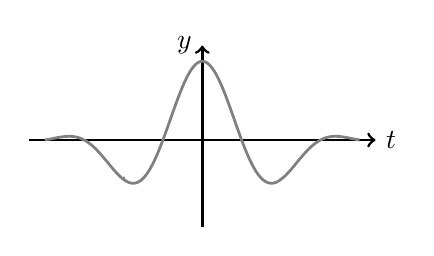
\begin{tikzpicture}[line width=1pt,domain=-2.2:2.2]
		\draw [->] (-2.2,0) -- (2.2,0) node[right] {$t$};
		\draw [->] (0,-1.1) -- (0,1.2) node[left] {$y$};
		%\draw plot[id=x] function{sin(3.1415926*x/8)*8/3.1415926/x*cos(3.1415926*x/8)/(1-(2*x/8)\^2)};
		\draw[domain=-2:2,samples=500,color=gray] plot(\x,{sin(pi*\x r)/(pi*\x)*cos(pi*\x r)/(1-\x*\x)});
	\end{tikzpicture}
	\caption{升余弦函数$(\alpha=0.5)$}
	\label{Figure:ddcode:rcos}
\end{figure}

	基带传输信号$x(t)$为:
\begin{equation}
x(t)=\sum_{n=0}^{\infty}u[n]c(t-nT_s)
\end{equation}
其中,$T_s=GT_c$为码元宽度。通带传输信号$\widetilde{x}(t)$为:
\begin{equation}
\label{passband_signal}
\widetilde{x}(t)=Re\{x(t)e^{j2\pi f_ct}\}
\end{equation}
其中,$f_c$为载波频率。

	通带信号$\widetilde{x}(t)$的频谱由$\phi(t)$,$T_c$和$f_c$决定。如前所述,$\phi(t)$为均方根升余弦函数,设其滚降因子为$\alpha$,那么$\phi(t)$的周期(也就是扩频码宽度)为:\[ T_c=\frac{\alpha+1}{f_h-f_l} \]其中$f_h-f_l=B$为传输带宽。综上,系统的传输率为:
\begin{equation}
R_b=\frac{\log_2M}{G}\times\frac{B}{1+\alpha}
\end{equation}
其中$M$为PSK调制阶数,如:BPSK($M=2$),QPSK($M=4$)。



\subsection{DD-SS的接收机}
	在实际水声信道中,传输信号会经过不同的路径传输至接收端即所谓的多途传播。水声信道随时间空间亦会发生缓慢变化,文献\cite{俊英1992水下声信道}给出了多途时变信道的系统函数:
\begin{equation}
h(t)=\sum_{p=1}^{N_p}A_p(t)\delta(t-\tau_p(t))
\end{equation}
式中$A_p(t)$为每条多途的幅度,$\tau_p(t)$为每条多途的延时。如果假设信道变化缓慢,在第$m$个分析时间间隔内可以认为$A_p(t)$和$\tau_p(t)$是常数$A_p[m]$和$\tau_p[m]$,那么系统函数可以简化为:
\begin{equation}
h(t,m)=\sum_{p=1}^{N_p}A_p[m]\delta(t-\tau_p[m])
\end{equation}

	根据上述假设,接收信号$\widetilde{r}(t)$为:
\begin{equation}
	\widetilde{r}(t,m)=\sum_{p=1}^{N_p}A_p[m]\widetilde{x}(t-\tau_p[m])
	\label{eq:ddcode:recv}
\end{equation}
\begin{figure}[htbp]
	\centering
	\begin{tikzpicture}[auto, thick, node distance=3cm, >=triangle 45]
	\draw
	node [input,name=in] {}
	node [block,right of=in, xshift=-0.6cm] (mod) {\wuhao 载波解调}
	node [block, right of=mod] (encode) {\wuhao 匹配滤波}
	node [block, right of=encode] (DS) {\wuhao 峰值检测}
	node [block,right of=DS] (cm) {\wuhao 二阶差分检测}
	node [output, right of=cm,xshift=-0.6cm] (out){}
	node [below of=encode, yshift=1.5cm] (ct) {}
	;
	\draw [->] (in)--(mod);
	\draw [->] (mod)--node[anchor=south] {$r(t)]$}(encode);
	\draw [->] (encode) -- node[anchor=south] {$y(t)$} (DS);
	\draw [->] (DS) -- node[anchor=south] {$y[n]$} (cm);
	\draw [->] (cm) -- (out);
	\draw [->] (ct) -- node[anchor=east] {$c(t)$} (encode);
	
	%label
	\draw 
	node [above right] at (in) {$\widetilde{r}(t)$}
	node [above left] at (out) {$d[n]$};
	
	\end{tikzpicture}
	\caption{DD-SS接收机系统框图}
	\label{Figure::ddcode:ddssrecv}
\end{figure}

\subsubsection{接收机解扩频}
	经过载波解调后的信号$r(t)$可以表示为:
\begin{equation}
	r(t)=\sum_{p=1}^{N_p}A_p[m]e^{-2j\pi f_c\tau_p[m]}c(t-mT_s-\tau)u[m]
\end{equation}
式中$u[m]$表示接收到的第$m$个符号,并且忽略了码间串扰。文献\cite{liu2014long}假设延时$\tau_p[m]$是线性变化的,即:\[ \tau_p[m+1] -\tau_p[m]~=~\tau_p[m]-\tau_p[m-1] \]

	在$N_p$个多途中,通过同步技术能够找到能量最大的第$q$条多途。则解扩后的信号$y[m]$为:
\begin{equation}
	y[m]=\int_{D_{q,m}}^{}r(t)c(t-mT_s-\tau_p[m])
\end{equation}结合上述假设,可以得到\citeup{liu2014long}:
\begin{equation}
	y[m]=A_q[m]e^{j2\pi f_c\tau_p[m]}u[m]
\end{equation}

\subsubsection{二阶差分检测}
	根据式(\ref{eq:ddcode:ddformula}),有:
\begin{equation}
\begin{split}
	d[n]&=\frac{v[n]}{v[n-1]} \\
	    &=\frac{u[n]}{u[n-1]}\times\frac{u[n-2]}{u[n-1]}
\end{split}
\end{equation}
类比上式并令$\phi_q[m]=-2\pi f_c \tau_q[m]$,进行如下变换:
\begin{equation}
\label{fu:ddcode:eq1}
\begin{split}
	z[m]=&\frac{y[m]}{y[m-1]}\times\frac{y[m-2]}{y[m-1]} \\
	=&\frac{A_q[m]e^{j\phi_q[m]} u[m]}{A_q[m-1]e^{j\phi_q[m-1]} u[m-1]} \times \frac{A_q[m-2]e^{j\phi_q[m-2]} u[m-2]}{A_q[m-1]e^{j\phi_q[m-1]} u[m-1]} \\
	=&\frac{A_q[m]A_q[m-2]}{A_q[m-1]A_q[m-1]}\times\frac{u[m]u[m-2]}{u[m-1]u[m-1]} \\
	&\times e^{j\left[(\phi_q[m]-\phi_q[m-1]) - (\phi_q[m-1] - \phi_q[m-2])\right]}
\end{split}
\end{equation}
由$\tau_p[m+1] -\tau_p[m]~=~\tau_p[m]-\tau_p[m-1]$可得\[ (\phi_q[m]-\phi_q[m-1]) - (\phi_q[m-1] - \phi_q[m-2]) = 0 \]则:
\begin{equation}
\begin{split}
z[m]&=\frac{A_q[m]A_q[m-2]}{A_q[m-1]A_q[m-1]}\times\frac{u[m]u[m-2]}{u[m-1]u[m-1]} \\
    &=\frac{A_q[m]A_q[m-2]}{A_q[m-1]A_q[m-1]}d[m]
\end{split}
\end{equation}
式中前一项为实数,并不影响PSK解调,因此:
\begin{equation}
d[m]=det \langle z[m] \rangle
\end{equation}
算子$det\langle \bullet \rangle$为PSK解调器。综上,可以将式(\ref{fu:ddcode:eq1})作为二阶差分检测器。

当考虑到多普勒影响时根据式(\ref{eq:ddcode:snd}),条件$(\phi_q[m]-\phi_q[m-1]) - (\phi_q[m-1] - \phi_q[m-2]) = 0$仍然成立。因此,结论不变。

\section{二阶差分检测抗干扰性能}
文献\cite{simon1992implementation}指出,二阶差分误码率可以表示为:
\begin{equation}
P_E=\frac{1}{2}exp\{ -\frac{E}{N_0}\left( 2+\frac{FT}{E/N_0}\right)^{}-1\}
\end{equation}
较一阶差分检测其检测性能要好3dB。
\begin{figure}[!htbp]
	\centering
	% This file was created by matlab2tikz.
%
%The latest updates can be retrieved from
%  http://www.mathworks.com/matlabcentral/fileexchange/22022-matlab2tikz-matlab2tikz
%where you can also make suggestions and rate matlab2tikz.
%
\definecolor{mycolor1}{rgb}{0.00000,0.44700,0.74100}%
\definecolor{mycolor2}{rgb}{0.85000,0.32500,0.09800}%
%
\begin{tikzpicture}

\begin{axis}[%
width=4.521in,
height=3.566in,
at={(0.758in,0.481in)},
scale only axis,
xmin=0,
xmax=20,
xlabel={SNR/dB},
xmajorgrids,
ymode=log,
ymin=1e-05,
ymax=1,
yminorticks=true,
ylabel={BER},
ymajorgrids,
yminorgrids,
axis background/.style={fill=white},
legend style={legend cell align=left,align=left,draw=white!15!black}
]
\addplot [color=mycolor1,solid,line width=0.8pt,mark=asterisk,mark options={solid}]
  table[row sep=crcr]{%
0	0.5\\
1	0.358265655286895\\
2	0.224664482058611\\
3	0.138226523314782\\
4	0.084506657703033\\
5	0.0515154017308821\\
6	0.0313551124140358\\
7	0.0190666632735226\\
8	0.0115872136205306\\
9	0.00703888800377979\\
10	0.00427465473984303\\
11	0.00259539451302863\\
12	0.00157555579922222\\
13	0.000956331029368268\\
14	0.000580414606959192\\
15	0.000352235103837373\\
16	0.00021374583448309\\
17	0.000129699536834225\\
18	7.86971247656689e-05\\
19	4.77487610977875e-05\\
20	2.89701449849997e-05\\
};
\addlegendentry{FT=1};

\addplot [color=mycolor2,line width=0.8pt,dashdotted]
  table[row sep=crcr]{%
0	0.5\\
1	0.389400391535702\\
2	0.256708559516296\\
3	0.162326233679175\\
4	0.100948258997328\\
5	0.0622572357220615\\
6	0.0382131434953841\\
7	0.0233853111919795\\
8	0.0142827503922752\\
9	0.00871118731974676\\
10	0.00530767323098834\\
11	0.00323148386204147\\
12	0.00196628614899365\\
13	0.00119589374870654\\
14	0.000727075296771791\\
15	0.000441913153467525\\
16	0.000268527038975621\\
17	0.000163136226901599\\
18	9.90918886595101e-05\\
19	6.01814025836066e-05\\
20	3.65453462897249e-05\\
};
\addlegendentry{FT=2};

\addplot [color=black,solid,line width=0.8pt,mark=o,mark options={solid}]
  table[row sep=crcr]{%
0	0.5\\
1	0.409365376538991\\
2	0.28235906100388\\
3	0.183939720585721\\
4	0.116753239545457\\
5	0.0730782785357713\\
6	0.0453589766447063\\
7	0.0280014181538868\\
8	0.0172219898306986\\
9	0.0105641399405916\\
10	0.00646745069447489\\
11	0.00395352702579672\\
12	0.00241397499691572\\
13	0.00147258872813418\\
14	0.000897652239573298\\
15	0.000546853837501227\\
16	0.000332978413354716\\
17	0.000202664634598067\\
18	0.000123306246479715\\
19	7.49997911318556e-05\\
20	4.560593201049e-05\\
};
\addlegendentry{FT=3};

\end{axis}
\end{tikzpicture}%
	\caption{二阶差分检测误码率曲线}
	\label{fig:ddcode:pe}
\end{figure}
\subsection{多普勒对DDSS系统的影响}
\label{sec:ddcode:dopuler}
如式(\ref{passband_signal})所示,通带传输信号为:
\[ \widetilde{x}(t)=Re\{x(t)e^{j2\pi f_ct}\} \]
经过多普勒作用之后的信号变成:
\begin{equation}
\widetilde{x}_D(t)=\widetilde{x}(Dt)=Re\{x(Dt)e^{j2\pi f_cDt}\}
\end{equation}
式中,$D=(1-v/c)/(1+v/c)\approx1-\alpha$\citeup{田坦2009声呐技术},$\alpha$称为多普勒因子。

\begin{figure}[htbp]
	\centering
%	\begin{tikzpicture}[>=stealth',node distance=2cm]
	% This file was created by matlab2tikz.
%
%The latest updates can be retrieved from
%  http://www.mathworks.com/matlabcentral/fileexchange/22022-matlab2tikz-matlab2tikz
%where you can also make suggestions and rate matlab2tikz.
%
\definecolor{mycolor1}{rgb}{0.00000,0.4,0.7}%
%
\begin{tikzpicture}

\begin{axis}[%
width=5.521in,
height=3.2in,
disabledatascaling,
at={(0.458in,0.5in)},
xmin=-0.001,
xmax=0.045,
xlabel={时间/$s$},
ymin=-1.1,
ymax=1.1,
ytick={-1, -0.5, ...,1}, xtick={0, 0.01, ...,0.04},
tick label style={/pgf/number format/fixed},
scaled ticks=false
]
\addplot [color=mycolor1,solid,forget plot]
  table[row sep=crcr]{%
0	-0.00937074173839967\\
4.16666666666667e-05	-0.443834535373538\\
8.33333333333333e-05	-0.111381355559634\\
0.000125	-0.203582703231228\\
0.000166666666666667	0.585158033349205\\
0.000208333333333333	0.733614729817017\\
0.00025	-0.867101082061622\\
0.000291666666666667	0.87796925651891\\
0.000333333333333333	-0.760990854225094\\
0.000375	0.530158296119893\\
0.000416666666666667	-0.21706665320692\\
0.000458333333333333	-0.134834314942189\\
0.0005	0.474224802250517\\
0.000541666666666667	-0.751345192946774\\
0.000583333333333333	0.953828463890035\\
0.000625	0.96909873115284\\
0.000666666666666667	-0.459475673284294\\
0.000708333333333333	-0.732976337969085\\
0.00075	0.927013082614822\\
0.000791666666666667	-0.994424325120626\\
0.000833333333333333	-0.917257716813808\\
0.000875	0.679191886854249\\
0.000916666666666667	-0.36523730929972\\
0.000958333333333333	0.00293578773480795\\
0.001	0.354618573323233\\
0.00104166666666667	-0.656090113803658\\
0.00108333333333333	0.859615981243003\\
0.001125	-0.936714300867531\\
0.00116666666666667	0.878990853144044\\
0.00120833333333333	-0.697247147485205\\
0.00125	-0.486742215642024\\
0.00129166666666667	0.90556821060086\\
0.00133333333333333	0.944609670224892\\
0.001375	-0.692137686571728\\
0.00141666666666667	0.442045703890428\\
0.00145833333333333	0.185414601931101\\
0.0015	0.175004071914193\\
0.00154166666666667	-0.450951801599212\\
0.00158333333333333	0.651679742907424\\
0.001625	-0.751214813949907\\
0.00166666666666667	0.739297350460878\\
0.00170833333333333	-0.623016469533713\\
0.00175	0.423909468089932\\
0.00179166666666667	-0.17531414034507\\
0.00183333333333333	-0.0839112078604397\\
0.001875	-0.390635395885828\\
0.00191666666666667	-0.601336078272586\\
0.00195833333333333	-0.346220209956931\\
0.002	-0.0707566146234127\\
0.00204166666666667	0.272572027020188\\
0.00208333333333333	0.625254769725648\\
0.002125	-0.490610037502596\\
0.00216666666666667	0.483916336297125\\
0.00220833333333333	-0.406085298366607\\
0.00225	0.275264925594783\\
0.00229166666666667	-0.116671731338754\\
0.00233333333333333	-0.0415967599861067\\
0.002375	0.174433644221127\\
0.00241666666666667	-0.262436457229966\\
0.00245833333333333	0.296029349981907\\
0.0025	0.872142724573447\\
0.00254166666666667	0.466565651153633\\
0.00258333333333333	0.453479622739717\\
0.002625	-0.187431290986977\\
0.00266666666666667	0.161042492243332\\
0.00270833333333333	0.857270697281293\\
0.00275	-0.0373097871048497\\
0.00279166666666667	-0.0264113662966324\\
0.00283333333333333	0.0702877811221857\\
0.002875	-0.083443445733534\\
0.00291666666666667	0.0634390029814915\\
0.00295833333333333	-0.0142904579284208\\
0.003	-0.0517448982429717\\
0.00304166666666667	0.118833436094644\\
0.00308333333333333	-0.169404660045855\\
0.003125	0.649102958908546\\
0.00316666666666667	0.394647090410866\\
0.00320833333333333	0.0843354001001103\\
0.00325	0.000703773946705364\\
0.00329166666666667	0.119563513692239\\
0.00333333333333333	-0.75098604392778\\
0.003375	-0.333852960088192\\
0.00341666666666667	0.384101657488498\\
0.00345833333333333	-0.374685274398409\\
0.0035	0.300355553970116\\
0.00354166666666667	-0.166935203831931\\
0.00358333333333333	-0.00918598160416272\\
0.003625	0.202267021841936\\
0.00366666666666667	-0.382245084508586\\
0.00370833333333333	0.518229299761112\\
0.00375	-0.906750626031815\\
0.00379166666666667	-0.589389395778977\\
0.00383333333333333	0.694015285959457\\
0.003875	0.588221404231372\\
0.00391666666666667	-0.674810967505104\\
0.00395833333333333	0.87301616885455\\
0.004	0.55121947189036\\
0.00404166666666667	-0.34907380291554\\
0.00408333333333333	0.0833743482578805\\
0.004125	0.207912278790793\\
0.00416666666666667	-0.481800277335027\\
0.00420833333333333	0.696074890814843\\
0.00425	-0.81562698882303\\
0.00429166666666667	0.819289517156165\\
0.00433333333333333	-0.70189370251966\\
0.004375	0.505990874895505\\
0.00441666666666667	0.160415664588265\\
0.00445833333333333	-0.210813882346447\\
0.0045	-0.484123027440736\\
0.00454166666666667	0.744139743132962\\
0.00458333333333333	-0.971061990626439\\
0.004625	-0.931760843318291\\
0.00466666666666667	0.826960538893991\\
0.00470833333333333	-0.600129341488298\\
0.00475	0.283173703035368\\
0.00479166666666667	0.0798172800898259\\
0.00483333333333333	-0.436302732154142\\
0.004875	0.733940268193808\\
0.00491666666666667	-0.927013082614847\\
0.00495833333333333	0.984405272669546\\
0.005	-0.899555918673878\\
0.00504166666666667	-0.701985822198916\\
0.00508333333333333	-0.387324566599413\\
0.005125	-0.0189359569300804\\
0.00516666666666667	-0.354618573323239\\
0.00520833333333333	0.656341285952238\\
0.00525	0.897157868439457\\
0.00529166666666667	-0.93671430086749\\
0.00533333333333333	0.878990853144022\\
0.005375	-0.697208090839951\\
0.00541666666666667	0.420475383701998\\
0.00545833333333333	-0.0911277357168279\\
0.0055	-0.242494178264663\\
0.00554166666666667	0.531528495835833\\
0.00558333333333333	-0.735977684738295\\
0.005625	0.828581671456642\\
0.00566666666666667	0.955968031971489\\
0.00570833333333333	0.561059209441094\\
0.00575	0.767498081426096\\
0.00579166666666667	-0.751214813949887\\
0.00583333333333333	0.739297350460906\\
0.005875	0.823567469598016\\
0.00591666666666667	-0.423909468089943\\
0.00595833333333333	0.175314140345047\\
0.006	0.0839112078604397\\
0.00604166666666667	-0.315551232858456\\
0.00608333333333333	0.486866727862084\\
0.006125	-0.577016300290828\\
0.00616666666666667	0.577503206341155\\
0.00620833333333333	-0.494912054522403\\
0.00625	0.347417870843798\\
0.00629166666666667	0.385270372295831\\
0.00633333333333333	-0.65168257885348\\
0.006375	-0.866265879557175\\
0.00641666666666667	0.275264925594801\\
0.00645833333333333	-0.116671731338723\\
0.0065	-0.121287306577278\\
0.00654166666666667	-0.174433644221039\\
0.00658333333333333	0.262436457229915\\
0.006625	-0.296029349981885\\
0.00666666666666667	0.275595588217515\\
0.00670833333333333	-0.211084927694484\\
0.00675	0.119662402380687\\
0.00679166666666667	-0.0218351963228034\\
0.00683333333333333	-0.0623861498589585\\
0.006875	0.11702476492103\\
0.00691666666666667	0.409322533987627\\
0.00695833333333333	0.545497537059105\\
0.007	0.284273845407951\\
0.00704166666666667	0.0834434457335881\\
0.00708333333333333	-0.0634390029815066\\
0.007125	-0.61175727379543\\
0.00716666666666667	-0.0517448982430466\\
0.00720833333333333	0.118833436094629\\
0.00725	-0.169404660045878\\
0.00729166666666667	0.188114155212145\\
0.00733333333333333	-0.165951956986259\\
0.007375	0.100855803133794\\
0.00741666666666667	-0.000703773946665323\\
0.00745833333333333	-0.119563513692282\\
0.0075	0.238749534782699\\
0.00754166666666667	-0.866294449545775\\
0.00758333333333333	-0.861386904724503\\
0.007625	-0.735860335834631\\
0.00766666666666667	-0.300355553970202\\
0.00770833333333333	0.166935203831908\\
0.00775	0.130277300782631\\
0.00779166666666667	0.202267021841929\\
0.00783333333333333	-0.38224508450864\\
0.007875	0.518229299761099\\
0.00791666666666667	-0.584658833652651\\
0.00795833333333333	0.565591189786708\\
0.008	-0.457360192297173\\
0.00804166666666667	0.271369287972144\\
0.00808333333333333	-0.0309722723362836\\
0.008125	-0.229273226558724\\
0.00816666666666667	0.652158340881349\\
0.00820833333333333	0.857141392083855\\
0.00825	0.942469623338902\\
0.00829166666666667	0.739624851730106\\
0.00833333333333333	-0.617524819401046\\
0.008375	0.443830086933362\\
0.00841666666666667	0.11138135555959\\
0.00845833333333333	0.203582703231231\\
0.0085	-0.500063438915205\\
0.00854166666666667	0.733621817862525\\
0.00858333333333333	-0.867101082061574\\
0.008625	0.877969256518885\\
0.00866666666666667	-0.760990854225241\\
0.00870833333333333	0.530158296119906\\
0.00875	-0.217066653206945\\
0.00879166666666667	-0.151859703135131\\
0.00883333333333333	-0.4716535064616\\
0.008875	0.611858596928011\\
0.00891666666666667	0.282674087637697\\
0.00895833333333333	0.0798172800897921\\
0.009	-0.459937152575062\\
0.00904166666666667	-0.732976337969084\\
0.00908333333333333	0.927013082614928\\
0.009125	-0.984405272669438\\
0.00916666666666667	0.897269781586829\\
0.00920833333333333	-0.679191886854199\\
0.00925	0.365237309299434\\
0.00929166666666667	-0.00293578773496347\\
0.00933333333333333	-0.354618573322956\\
0.009375	0.656090113803901\\
0.00941666666666667	-0.859954211441074\\
0.00945833333333333	-0.994013200795355\\
0.0095	-0.950177602100207\\
0.00954166666666667	-0.77262255274246\\
0.00958333333333333	0.420475383702111\\
0.009625	-0.0911009846717131\\
0.00966666666666667	0.236164858360189\\
0.00970833333333333	-0.531528495836067\\
0.00975	0.735977684738082\\
0.00979166666666667	-0.828584446694664\\
0.00983333333333333	0.79981083945368\\
0.009875	-0.658243366153204\\
0.00991666666666667	0.42830323967503\\
0.00995833333333333	-0.147225025775944\\
0.01	-0.142225502715716\\
0.0100416666666667	0.397461668674417\\
0.0100833333333333	0.729008083036805\\
0.010125	-0.674709283350112\\
0.0101666666666667	-0.939941156467618\\
0.0102083333333333	0.559364789730579\\
0.01025	-0.380294243995384\\
0.0102916666666667	-0.346220209956774\\
0.0103333333333333	-0.0707566146234839\\
0.010375	0.272572027019914\\
0.0104166666666667	-0.418248061722646\\
0.0104583333333333	0.490610037502881\\
0.0105	-0.483916336297021\\
0.0105416666666667	0.406085298366528\\
0.0105833333333333	-0.275264925594739\\
0.010625	0.116671731338672\\
0.0106666666666667	0.0415967599858738\\
0.0107083333333333	0.214552020034672\\
0.01075	-0.262436457230139\\
0.0107916666666667	-0.747750630269527\\
0.0108333333333333	0.275595588217298\\
0.010875	-0.211084927694525\\
0.0109166666666667	-0.755899551302778\\
0.0109583333333333	0.0218351963228309\\
0.011	0.0623861498589725\\
0.0110416666666667	-0.117024764921315\\
0.0110833333333333	0.133808993318719\\
0.011125	-0.112077793926414\\
0.0111666666666667	0.0603753346901406\\
0.0112083333333333	0.00726951253062244\\
0.01125	-0.0730250563856385\\
0.0112916666666667	0.119424751158449\\
0.0113333333333333	-0.347164477256412\\
0.011375	-0.0253296953003689\\
0.0114166666666667	0.300916379781852\\
0.0114583333333333	0.041771345897337\\
0.0115	-0.139935088348218\\
0.0115416666666667	0.88445000118088\\
0.0115833333333333	0.283962001637155\\
0.011625	-0.293596897859749\\
0.0116666666666667	0.248445292603831\\
0.0117083333333333	-0.149885058638445\\
0.01175	0.00997161966853686\\
0.0117916666666667	0.150630458233264\\
0.0118333333333333	-0.305711816939558\\
0.011875	0.427399583454888\\
0.0119166666666667	-0.491618576936734\\
0.0119583333333333	0.793359307821411\\
0.012	0.393557940440858\\
0.0120416666666667	-0.267383902465563\\
0.0120833333333333	-0.0242210662451737\\
0.012125	-0.20629165361296\\
0.0121666666666667	0.694015285959553\\
0.0122083333333333	0.588221404231423\\
0.01225	-0.674810967504681\\
0.0122916666666667	0.663960128983611\\
0.0123333333333333	-0.551219471890708\\
0.012375	0.349073802915594\\
0.0124166666666667	-0.083374348257627\\
0.0124583333333333	-0.207912278791151\\
0.0125	0.481800277335147\\
0.0125416666666667	-0.696074890814404\\
0.0125833333333333	0.967483657173889\\
0.012625	0.907340723378994\\
0.0126666666666667	0.585133421437735\\
0.0127083333333333	0.733614729816959\\
0.01275	-0.867101082061577\\
0.0127916666666667	0.955220417887304\\
0.0128333333333333	0.761068784644828\\
0.012875	-0.530158296119923\\
0.0129166666666667	0.21706665320646\\
0.0129583333333333	0.134834314942231\\
0.013	-0.474224802250212\\
0.0130416666666667	0.751345192946835\\
0.0130833333333333	-0.924234667318317\\
0.013125	0.96646761471854\\
0.0131666666666667	-0.870775330385162\\
0.0132083333333333	0.654800993858498\\
0.01325	0.321595872616695\\
0.0132916666666667	-0.999999999999762\\
0.0133333333333333	-0.917257716813609\\
0.013375	0.679191886854495\\
0.0134166666666667	-0.364370065456731\\
0.0134583333333333	-0.0189359569301052\\
0.0135	-0.354618573322854\\
0.0135416666666667	0.656090113803963\\
0.0135833333333333	-0.859615981243244\\
0.013625	0.936714300867135\\
0.0136666666666667	-0.878990853144193\\
0.0137083333333333	0.69720809083999\\
0.01375	-0.420475383701903\\
0.0137916666666667	0.0911277357171653\\
0.0138333333333333	0.242626106818347\\
0.013875	0.570226144313535\\
0.0139166666666667	-0.438981718473105\\
0.0139583333333333	-0.185414601930883\\
0.014	-0.175004071914335\\
0.0140416666666667	0.45095516526509\\
0.0140833333333333	0.767498081426015\\
0.014125	-0.751214813949555\\
0.0141666666666667	0.739297350460858\\
0.0142083333333333	-0.623016469534152\\
0.01425	0.423909468090028\\
0.0142916666666667	-0.175314140344866\\
0.0143333333333333	-0.0839112078605916\\
0.014375	0.315551232858333\\
0.0144166666666667	-0.486866727862117\\
0.0144583333333333	0.577016300290538\\
0.0145	0.908873650203915\\
0.0145416666666667	0.477848370958851\\
0.0145833333333333	0.625254769725566\\
0.014625	-0.490610037502964\\
0.0146666666666667	0.483916336297098\\
0.0147083333333333	0.866265879557242\\
0.01475	-0.27526492559506\\
0.0147916666666667	0.116671731338278\\
0.0148333333333333	0.0415967599860857\\
0.014875	-0.174433644220373\\
0.0149166666666667	0.262436457230016\\
0.0149583333333333	-0.296029349982121\\
0.015	0.275595588217493\\
0.0150416666666667	-0.211084927694556\\
0.0150833333333333	0.119662402380455\\
0.015125	0.531665801256313\\
0.0151666666666667	0.235015625552087\\
0.0152083333333333	-0.094431375775034\\
0.01525	0.133808993319191\\
0.0152916666666667	-0.112077793926801\\
0.0153333333333333	-0.831786910264163\\
0.015375	-0.00726951253075475\\
0.0154166666666667	0.0730250563859364\\
0.0154583333333333	-0.119424751158442\\
0.0155	0.133631372836115\\
0.0155416666666667	-0.108534555776701\\
0.0155833333333333	0.046865577540134\\
0.015625	0.0417713458976151\\
0.0156666666666667	-0.139935088348609\\
0.0157083333333333	0.227384235967349\\
0.01575	-0.85600687794879\\
0.0157916666666667	-0.707628229967104\\
0.0158333333333333	-0.459226320652198\\
0.015875	-0.149885058639113\\
0.0159166666666667	0.00997161966846211\\
0.0159583333333333	0.5019001501584\\
0.016	0.305711816939339\\
0.0160416666666667	-0.427399583454677\\
0.0160833333333333	0.491618576936873\\
0.016125	-0.482064745104099\\
0.0161666666666667	0.393557940441007\\
0.0162083333333333	-0.234360727788437\\
0.01625	0.0242210662447192\\
0.0162916666666667	0.206291653613066\\
0.0163333333333333	-0.422267455852039\\
0.016375	0.879445194428698\\
0.0164166666666667	0.784745327303184\\
0.0164583333333333	-0.357978290246381\\
0.0165	-0.470690862628216\\
0.0165416666666667	0.654998825040765\\
0.0165833333333333	-0.942469623338787\\
0.016625	-0.739624851730308\\
0.0166666666666667	0.617524819401211\\
0.0167083333333333	-0.39858253857711\\
0.01675	0.11135516712674\\
0.0167916666666667	0.203582703231347\\
0.0168333333333333	-0.500063438914729\\
0.016875	0.733621817862242\\
0.0169166666666667	-0.867101082061893\\
0.0169583333333333	0.877969256519041\\
0.017	-0.814174708782804\\
0.0170416666666667	-0.556567554163022\\
0.0170833333333333	-0.219108194029469\\
0.017125	0.134841452661839\\
0.0171666666666667	-0.474224802250093\\
0.0172083333333333	0.783404679335018\\
0.01725	0.924407206745726\\
0.0172916666666667	-0.966467614718133\\
0.0173333333333333	0.870775330384861\\
0.017375	-0.648228658110935\\
0.0174166666666667	0.329639772876093\\
0.0174583333333333	0.0391285842732065\\
0.0175	-0.401849844165942\\
0.0175416666666667	0.703783338004215\\
0.0175833333333333	-0.901840049031885\\
0.017625	0.969193975761192\\
0.0176666666666667	0.928807720512291\\
0.0177083333333333	0.680219847740102\\
0.01775	0.897157868439879\\
0.0177916666666667	-0.936714300867154\\
0.0178333333333333	0.878766439719344\\
0.017875	0.772622552743123\\
0.0179166666666667	-0.420475383702286\\
0.0179583333333333	0.0911277357168807\\
0.018	0.242494178264653\\
0.0180416666666667	-0.531528495836207\\
0.0180833333333333	0.735977684738255\\
0.018125	-0.828584446694261\\
0.0181666666666667	0.799810839453648\\
0.0182083333333333	-0.658243366153837\\
0.01825	0.428269417219937\\
0.0182916666666667	0.243917991916347\\
0.0183333333333333	0.850662785687664\\
0.018375	0.823567469598309\\
0.0184166666666667	-0.423909468090246\\
0.0184583333333333	0.175314140344698\\
0.0185	-0.0562779915881787\\
0.0185416666666667	0.315551232858056\\
0.0185833333333333	-0.486866727862203\\
0.018625	0.577016300290824\\
0.0186666666666667	-0.577503206341076\\
0.0187083333333333	0.494912054522731\\
0.01875	-0.347417870843627\\
0.0187916666666667	0.162071851779463\\
0.0188333333333333	0.0298196993058283\\
0.018875	-0.198988910713123\\
0.0189166666666667	-0.560821093896711\\
0.0189583333333333	-0.47371816987426\\
0.019	-0.121287306577374\\
0.0190416666666667	-0.174433644220766\\
0.0190833333333333	0.26243645722983\\
0.019125	0.747750630269842\\
0.0191666666666667	-0.275595588217721\\
0.0192083333333333	0.211084927694076\\
0.01925	-0.119662402380304\\
0.0192916666666667	0.0218351963228586\\
0.0193333333333333	0.0623861498589947\\
0.019375	-0.117024764920615\\
0.0194166666666667	0.133808993318848\\
0.0194583333333333	-0.112077793927228\\
0.0195	0.0603753346897798\\
0.0195416666666667	0.880242454343128\\
0.0195833333333333	0.806588153054106\\
0.019625	0.619980671375045\\
0.0196666666666667	0.133631372836336\\
0.0197083333333333	-0.108534555776574\\
0.01975	-0.300916379781532\\
0.0197916666666667	-0.0417713458971433\\
0.0198333333333333	0.139935088348982\\
0.019875	-0.227384235967264\\
0.0199166666666667	0.283962001636851\\
0.0199583333333333	-0.293596897859797\\
0.02	0.248445292603852\\
0.0200416666666667	-0.149885058638464\\
0.0200833333333333	0.00997161966909202\\
0.020125	0.150630458233879\\
0.0201666666666667	-0.745517086670413\\
0.0202083333333333	-0.427399583454308\\
0.02025	0.902736020129692\\
0.0202916666666667	0.482064745104571\\
0.0203333333333333	-0.393557940440517\\
0.020375	0.26738390246571\\
0.0204166666666667	0.0242210662449352\\
0.0204583333333333	0.206291653613345\\
0.0205	-0.422267455852138\\
0.0205416666666667	0.588221404231127\\
0.0205833333333333	-0.674810967505115\\
0.020625	0.663960128983523\\
0.0206666666666667	-0.551219471890266\\
0.0207083333333333	0.349073802915996\\
0.02075	-0.0833743482576647\\
0.0207916666666667	-0.316355405152339\\
0.0208333333333333	-0.608424410822591\\
0.020875	-0.443840441404339\\
0.0209166666666667	-0.1113813555595\\
0.0209583333333333	-0.20358270323137\\
0.021	0.585158033349258\\
0.0210416666666667	0.733614729816634\\
0.0210833333333333	-0.867101082062149\\
0.021125	0.87796925651922\\
0.0211666666666667	-0.760990854224858\\
0.0212083333333333	0.530158296119822\\
0.02125	-0.21706665320697\\
0.0212916666666667	-0.134834314942373\\
0.0213333333333333	0.47422480225003\\
0.021375	-0.751345192946756\\
0.0214166666666667	0.953828463890416\\
0.0214583333333333	0.969098731152711\\
0.0215	-0.459475673284273\\
0.0215416666666667	-0.732976337969228\\
0.0215833333333333	0.927013082614925\\
0.021625	-0.994424325120787\\
0.0216666666666667	-0.917257716813649\\
0.0217083333333333	0.679191886853903\\
0.02175	-0.365237309300074\\
0.0217916666666667	0.00293578773495749\\
0.0218333333333333	0.354618573323502\\
0.021875	-0.656090113803862\\
0.0219166666666667	0.859615981242816\\
0.0219583333333333	-0.936714300867576\\
0.022	0.878990853143792\\
0.0220416666666667	-0.697247147485171\\
0.0220833333333333	-0.486831539821885\\
0.022125	-0.13408337663754\\
0.0221666666666667	0.23616485836007\\
0.0222083333333333	-0.531528495835499\\
0.02225	0.735928824088357\\
0.0222916666666667	0.956854344291464\\
0.0223333333333333	-0.799810839453606\\
0.022375	0.658243366153683\\
0.0224166666666667	-0.428303239674881\\
0.0224583333333333	0.14722502577546\\
0.0225	0.142225502715449\\
0.0225416666666667	-0.397461668674523\\
0.0225833333333333	0.582705035162354\\
0.022625	-0.674709283349798\\
0.0226666666666667	0.664392265199662\\
0.0227083333333333	0.850311416186756\\
0.02275	-0.44608829392052\\
0.0227916666666667	-0.848293871370049\\
0.0228333333333333	0.57750320634134\\
0.022875	-0.494912054522404\\
0.0229166666666667	-0.659070008974684\\
0.0229583333333333	0.162071851779587\\
0.023	0.0298196993062238\\
0.0230416666666667	-0.198988910712743\\
0.0230833333333333	0.321042267616559\\
0.023125	-0.382025323072788\\
0.0231666666666667	0.378170339473888\\
0.0232083333333333	-0.317120886255686\\
0.02325	0.21514598935622\\
0.0232916666666667	-0.0937962602164605\\
0.0233333333333333	-0.173559754828923\\
0.023375	0.559892464885738\\
0.0234166666666667	0.755899551302862\\
0.0234583333333333	-0.0218351963230837\\
0.0235	-0.0623861498588671\\
0.0235416666666667	-0.0944313757745091\\
0.0235833333333333	0.133808993318472\\
0.023625	-0.11207779392701\\
0.0236666666666667	0.0603753346899293\\
0.0237083333333333	0.00726951253130009\\
0.02375	-0.0730250563856659\\
0.0237916666666667	0.119424751158036\\
0.0238333333333333	-0.133631372836682\\
0.023875	0.10853455577666\\
0.0239166666666667	-0.0468655775399338\\
0.0239583333333333	-0.58563300303663\\
0.024	-0.790139511719128\\
0.0240416666666667	-0.884450001181273\\
0.0240833333333333	-0.283962001636417\\
0.024125	0.293596897859735\\
0.0241666666666667	-0.459226320652836\\
0.0242083333333333	-0.149885058638498\\
0.02425	0.00997161966882413\\
0.0242916666666667	0.150630458233766\\
0.0243333333333333	-0.305711816939921\\
0.024375	0.427399583454348\\
0.0244166666666667	-0.491618576936376\\
0.0244583333333333	0.482064745104537\\
0.0245	-0.393557940440838\\
0.0245416666666667	0.234360727788153\\
0.0245833333333333	0.0771978132795793\\
0.024625	0.413075463859197\\
0.0246666666666667	0.694015285959691\\
0.0247083333333333	0.588221404230829\\
0.02475	-0.674810967505352\\
0.0247916666666667	0.873016168854584\\
0.0248333333333333	0.551219471889883\\
0.024875	-0.349073802915868\\
0.0249166666666667	0.0833743482581278\\
0.0249583333333333	0.207912278790597\\
0.025	-0.481800277335058\\
0.0250416666666667	0.696074890815066\\
0.0250833333333333	-0.815626988822424\\
0.025125	0.819289517155985\\
0.0251666666666667	-0.701893702519605\\
0.0252083333333333	0.505990874895501\\
0.02525	0.175216784503941\\
0.0252916666666667	0.210800506513125\\
0.0253333333333333	0.484123027440897\\
0.025375	-0.744139743132536\\
0.0254166666666667	0.971061990626064\\
0.0254583333333333	0.931760843318388\\
0.0255	-0.826960538893994\\
0.0255416666666667	0.600129341488299\\
0.0255833333333333	-0.283173703035476\\
0.025625	-0.0798172800900658\\
0.0256666666666667	0.436302732154221\\
0.0257083333333333	-0.733940268193254\\
0.02575	0.927013082614693\\
0.0257916666666667	-0.984405272669468\\
0.0258333333333333	0.899555918673537\\
0.025875	0.702776887366439\\
0.0259166666666667	-0.898442197906754\\
0.0259583333333333	-0.993727875594898\\
0.026	0.898418264492812\\
0.0260416666666667	-0.700877979350954\\
0.0260833333333333	-0.433653280735853\\
0.026125	0.0608085386902092\\
0.0261666666666667	0.287118998248946\\
0.0262083333333333	-0.586286507853236\\
0.02625	0.79554746472172\\
0.0262916666666667	-0.886332570588526\\
0.0263333333333333	0.848915432572501\\
0.026375	-0.692137686571011\\
0.0264166666666667	0.442045050958973\\
0.0264583333333333	-0.137943999687218\\
0.0265	0.175671210992582\\
0.0265416666666667	-0.710870727094883\\
0.0265833333333333	-0.57122249766093\\
0.026625	0.147225025776106\\
0.0266666666666667	0.142225502714935\\
0.0267083333333333	0.455516359640321\\
0.02675	-0.582705035162246\\
0.0267916666666667	0.674709283349785\\
0.0268333333333333	-0.664392265199598\\
0.026875	0.559364789730205\\
0.0269166666666667	-0.380294243995487\\
0.0269583333333333	0.158274641110189\\
0.027	0.0707566146236854\\
0.0270416666666667	-0.272572027020249\\
0.0270833333333333	0.418248061722525\\
0.027125	0.826189084700533\\
0.0271666666666667	0.228231756947468\\
0.0272083333333333	-0.270750502157544\\
0.02725	0.321042267616625\\
0.0272916666666667	-0.382025323072184\\
0.0273333333333333	-0.872563078532504\\
0.027375	0.317120886255979\\
0.0274166666666667	-0.215145989356289\\
0.0274583333333333	0.0937962602167469\\
0.0275	0.023823140972709\\
0.0275416666666667	-0.117758113962367\\
0.0275833333333333	0.174168422886909\\
0.027625	-0.187431290986507\\
0.0276666666666667	0.161042492243427\\
0.0277083333333333	-0.105651143464918\\
0.02775	-0.763099581698022\\
0.0277916666666667	-0.562330052281932\\
0.0278333333333333	-0.284273845407737\\
0.027875	-0.0834434457340036\\
0.0279166666666667	0.0634390029810646\\
0.0279583333333333	0.611757273795581\\
0.028	0.0517448982426641\\
0.0280416666666667	-0.118833436094747\\
0.0280833333333333	0.169404660045947\\
0.028125	-0.18811415521234\\
0.0281666666666667	0.165951956986649\\
0.0282083333333333	-0.100855803133592\\
0.02825	0.000703773946258189\\
0.0282916666666667	0.119563513691987\\
0.0283333333333333	-0.238749534782392\\
0.028375	0.866294449545832\\
0.0284166666666667	0.723147264776899\\
0.0284583333333333	0.501900150158187\\
0.0285	0.305711816939243\\
0.0285416666666667	-0.42739958345459\\
0.0285833333333333	0.90273602013031\\
0.028625	0.482064745104495\\
0.0286666666666667	-0.393557940440457\\
0.0287083333333333	0.234360727788318\\
0.02875	-0.0242210662451884\\
0.0287916666666667	-0.206291653612854\\
0.0288333333333333	0.42226745585208\\
0.028875	-0.588221404231868\\
0.0289166666666667	0.674810967505459\\
0.0289583333333333	-0.66396012898342\\
0.029	0.679471330303792\\
0.0290416666666667	0.388806614254134\\
0.0290833333333333	0.0405277361845246\\
0.029125	-0.207897989540245\\
0.0291666666666667	0.481800277335229\\
0.0292083333333333	-0.859486368195791\\
0.02925	-0.815651072601128\\
0.0292916666666667	0.819289517155911\\
0.0293333333333333	-0.701893702519874\\
0.029375	0.477128418075314\\
0.0294166666666667	-0.17507857927401\\
0.0294583333333333	-0.161778192495717\\
0.0295	0.484011962326981\\
0.0295416666666667	-0.744139743133196\\
0.0295833333333333	0.901873246519078\\
0.029625	-0.985422915209445\\
0.0296666666666667	-0.860404764388161\\
0.0297083333333333	-0.61189191363786\\
0.02975	-0.282674087638269\\
0.0297916666666667	-0.0798172800896832\\
0.0298333333333333	0.459937152575377\\
0.029875	0.732976337968992\\
0.0299166666666667	-0.927013082614601\\
0.0299583333333333	0.98440527267023\\
0.03	-0.897269781586876\\
0.0300416666666667	0.679191886854193\\
0.0300833333333333	-0.365237309299815\\
0.030125	0.0029357877348745\\
0.0301666666666667	0.35461857332308\\
0.0302083333333333	-0.656090113803349\\
0.03025	0.859954211441466\\
0.0302916666666667	0.994013200795964\\
0.0303333333333333	0.950177602100064\\
0.030375	0.772622552742955\\
0.0304166666666667	-0.420475383702306\\
0.0304583333333333	0.0911009846711748\\
0.0305	-0.236164858359654\\
0.0305416666666667	0.531528495835457\\
0.0305833333333333	-0.735977684738862\\
0.030625	0.828584446694725\\
0.0306666666666667	-0.799810839453444\\
0.0307083333333333	0.658243366153565\\
0.03075	-0.428303239674749\\
0.0307916666666667	0.147225025775923\\
0.0308333333333333	0.14222550271506\\
0.030875	-0.397461668674884\\
0.0309166666666667	-0.729008083037276\\
0.0309583333333333	-0.344047093135878\\
0.031	0.0562779915880808\\
0.0310416666666667	-0.315551232858559\\
0.0310833333333333	0.486866727862039\\
0.031125	0.848293871369787\\
0.0311666666666667	-0.577503206340682\\
0.0312083333333333	0.494912054522398\\
0.03125	-0.347417870844387\\
0.0312916666666667	0.162071851780121\\
0.0313333333333333	0.0298196993062719\\
0.031375	-0.198988910713203\\
0.0314166666666667	0.321042267616434\\
0.0314583333333333	-0.382025323072345\\
0.0315	0.378170339473837\\
0.0315416666666667	0.851901813754914\\
0.0315833333333333	-0.141085270096515\\
0.031625	-0.747750630269577\\
0.0316666666666667	0.275595588217692\\
0.0317083333333333	-0.211084927694486\\
0.03175	-0.75589955130312\\
0.0317916666666667	0.0218351963229839\\
0.0318333333333333	0.062386149859799\\
0.031875	-0.117024764920884\\
0.0319166666666667	0.133808993318071\\
0.0319583333333333	-0.112077793926682\\
0.032	0.0603753346903071\\
0.0320416666666667	0.00726951253063295\\
0.0320833333333333	-0.0730250563851857\\
0.032125	0.11942475115886\\
0.0321666666666667	-0.347164477256647\\
0.0322083333333333	-0.0253296953005174\\
0.03225	0.300916379781982\\
0.0322916666666667	0.0417713458967204\\
0.0323333333333333	-0.139935088348655\\
0.032375	0.884450001180867\\
0.0324166666666667	0.283962001637078\\
0.0324583333333333	-0.293596897860083\\
0.0325	0.248445292603824\\
0.0325416666666667	-0.149885058637959\\
0.0325833333333333	0.00997161966883917\\
0.032625	0.150630458233248\\
0.0326666666666667	-0.305711816939576\\
0.0327083333333333	0.427399583454548\\
0.03275	-0.491618576936921\\
0.0327916666666667	0.793359307821756\\
0.0328333333333333	0.320448698613316\\
0.032875	-0.866607471449702\\
0.0329166666666667	-0.584658833652803\\
0.0329583333333333	0.565591189786536\\
0.033	-0.616225448939386\\
0.0330416666666667	-0.271369287972111\\
0.0330833333333333	0.0309722723366232\\
0.033125	0.229273226558232\\
0.0331666666666667	-0.470690862628414\\
0.0332083333333333	0.65499882504159\\
0.03325	-0.750842063493869\\
0.0332916666666667	0.739624851729934\\
0.0333333333333333	-0.617524819401352\\
0.033375	0.398582538577213\\
0.0334166666666667	-0.101017219800808\\
0.0334583333333333	0.203584680574106\\
0.0335	-0.585158033349385\\
0.0335416666666667	-0.733614729816907\\
0.0335833333333333	0.867101082061222\\
0.033625	-0.955220417887427\\
0.0336666666666667	-0.76106878464474\\
0.0337083333333333	0.530158296119939\\
0.03375	-0.217066653207443\\
0.0337916666666667	-0.134834314942455\\
0.0338333333333333	0.474224802250472\\
0.033875	-0.751345192946155\\
0.0339166666666667	0.924234667318236\\
0.0339583333333333	-0.96646761471858\\
0.034	0.870775330385005\\
0.0340416666666667	-0.654800993859215\\
0.0340833333333333	-0.321595872616977\\
0.034125	1\\
0.0341666666666667	0.917257716814149\\
0.0342083333333333	-0.679191886853885\\
0.03425	0.364370065456657\\
0.0342916666666667	0.0189359569301919\\
0.0343333333333333	0.354618573322922\\
0.034375	-0.656090113803224\\
0.0344166666666667	0.859615981242718\\
0.0344583333333333	-0.936714300867795\\
0.0345	0.878990853143902\\
0.0345416666666667	-0.697208090839496\\
0.0345833333333333	0.420475383701979\\
0.034625	-0.0911277357172837\\
0.0346666666666667	-0.242626106818662\\
0.0347083333333333	-0.570226144312594\\
0.03475	0.438981718472531\\
0.0347916666666667	0.185414601931485\\
0.0348333333333333	0.175004071913938\\
0.034875	-0.450955165265507\\
0.0349166666666667	-0.767498081425864\\
0.0349583333333333	0.751214813949772\\
0.035	-0.739297350460823\\
0.0350416666666667	0.623016469533533\\
0.0350833333333333	-0.423909468090047\\
0.035125	0.175314140345421\\
0.0351666666666667	0.0839112078604517\\
0.0352083333333333	-0.315551232859022\\
0.03525	0.48686672786198\\
0.0352916666666667	-0.577016300290586\\
0.0353333333333333	-0.908873650203786\\
0.035375	0.494912054522052\\
0.0354166666666667	0.659070008975092\\
0.0354583333333333	-0.162071851780284\\
0.0355	-0.0298196993067187\\
0.0355416666666667	-0.27075050215686\\
0.0355833333333333	0.321042267616081\\
0.035625	-0.382025323072616\\
0.0356666666666667	0.378170339473814\\
0.0357083333333333	-0.317120886256149\\
0.03575	0.215145989356766\\
0.0357916666666667	-0.0937962602165414\\
0.0358333333333333	-0.0238231409731951\\
0.035875	0.117758113961743\\
0.0359166666666667	-0.174168422887271\\
0.0359583333333333	-0.691707541184591\\
0.036	0.161042492243267\\
0.0360416666666667	0.857270697281427\\
0.0360833333333333	-0.0373097871047193\\
0.036125	-0.026411366297149\\
0.0361666666666667	0.284273845408187\\
0.0362083333333333	0.0834434457330157\\
0.03625	-0.0634390029814641\\
0.0362916666666667	0.0142904579284623\\
0.0363333333333333	0.0517448982431204\\
0.036375	-0.118833436094522\\
0.0364166666666667	0.169404660046319\\
0.0364583333333333	-0.188114155212734\\
0.0365	0.165951956985743\\
0.0365416666666667	-0.100855803133796\\
0.0365833333333333	-0.239796019537138\\
0.036625	-0.532452515491923\\
0.0366666666666667	-0.459226320653241\\
0.0367083333333333	-0.149885058638393\\
0.03675	0.00997161966873778\\
0.0367916666666667	0.5019001501576\\
0.0368333333333333	0.305711816939542\\
0.036875	-0.42739958345504\\
0.0369166666666667	0.491618576936705\\
0.0369583333333333	-0.482064745104118\\
0.037	0.393557940440874\\
0.0370416666666667	-0.234360727787326\\
0.0370833333333333	0.024221066246099\\
0.037125	0.206291653612905\\
0.0371666666666667	-0.422267455852366\\
0.0372083333333333	0.879445194428448\\
0.03725	0.784745327303535\\
0.0372916666666667	-0.357978290245697\\
0.0373333333333333	-0.470690862628089\\
0.037375	0.654998825041325\\
0.0374166666666667	-0.94246962333846\\
0.0374583333333333	-0.739624851729688\\
0.0375	0.617524819401337\\
0.0375416666666667	-0.398582538577099\\
0.0375833333333333	0.111355167127108\\
0.037625	0.20358270323029\\
0.0376666666666667	-0.500063438915213\\
0.0377083333333333	0.733621817862425\\
0.03775	-0.867101082061113\\
0.0377916666666667	0.877969256519072\\
0.0378333333333333	-0.814174708783347\\
0.037875	-0.543588749824731\\
};
\end{axis}
\end{tikzpicture}%
	%\draw [->] (0,0)--(4,0);
	%\draw [->] (2,-0.2)--(2,1.5) node [below,xshift=-0.5cm] {$a(f)$};
	%\draw[xshift=2cm] plot[samples=300,domain=-1.8:1.8,id=paipin] function{abs(sin(2*pi*x)/(2*pi*x))};
	%\draw[xshift=2cm] node at (0.5cm,-0.5cm) {$\frac{B_a}{2}$};
	%\draw[xshift=2cm] node at (-0.5cm,-0.5cm) {$\text{-}\frac{B_a}{2}$};
	
%	\end{tikzpicture}
	\caption{有多普勒信号解调}
	\label{fig::paiping}
\end{figure}

在接收端不对$\alpha$进行估计,仍然以载波频率$f_c$对接受信号进行解调。解调后的信号将会混入一个频率为$\alpha f_c$的拍频。如图\ref{fig::paiping}所示,拍频的包络宽度为$\alpha f_c$频率信号周期的一半,即:
\begin{equation}
\label{equ:ddcode:td}
T_D=\frac{1}{2\alpha f_c}
\end{equation}
解调信号在相邻两个包络之间相位发生翻转。

图\ref{fig::pnwdopler}展示了多普勒大小与PN序列长短的关系。在解扩时,如果PN序列长度比$T_D$大,接收信号在中间位置发生了相位翻转,积分得到的峰值变小干扰增大,更严重的将会出现错峰(如图\ref{fig::pnwdopler}(a)所示)。对于相同大小的多普勒,当PN序列越短(比$T_D$小得多)时,更有利于解扩(如图\ref{fig::pnwdopler}(b)所示)。

长度为$G$码元宽度为$T_c$的PN序列,其时间长度为\[T_G=GT_c=\frac{2G}{B}\]式中,$B$为系统传输带宽。若要更好的解扩,需满足$T_G<<T_D$,即:
\[
\alpha << \frac{B}{4\alpha f_c}
\]
则有系统容忍最大的多普勒为:
\begin{equation}
\alpha_{max} \varpropto \frac{B}{4\alpha f_c}
\end{equation}
因此,降低载波频率、增大带宽、减小PN序列长度均有利于系统抵抗多普勒。

\begin{figure}[htbp]
	\centering
	\begin{minipage}{0.8\textwidth}
		\centering
		\subfigure[多普勒较大时]{
			\begin{tikzpicture}[>=stealth',node distance=2cm]
	\draw [->] (-0.1,0)--(8.5,0) node [right=3pt] {$t$};
	\draw [->] (0,-1.5)--(0,1.5);
	\draw plot[samples=300,domain=0:8,id=pai_a] function{sin(pi*x)};
	\draw plot[samples=300,domain=0:8,id=pai_b] function{-sin(pi*x)};
	\draw [|<->|,dashed] (0,1) --node[above] {\xiaowu 短PN序列} (1.7,1);
	
\end{tikzpicture}
		}
	\end{minipage}
	\begin{minipage}{0.8\textwidth}
		\centering
		\subfigure[多普勒较小时]{
			\begin{tikzpicture}[>=stealth',node distance=2cm]
	\draw [->] (-0.1,0)--(8.5,0) node [right=3pt] {$t$};
	\draw [->] (0,-1.5)--(0,1.5);
	\draw plot[samples=300,domain=0:8,id=pai_ba] function{sin(0.25*pi*x)};
	\draw plot[samples=300,domain=0:8,id=pai_bb] function{-sin(0.25*pi*x)};
	\draw [|<->|,dashed] (0,0.8) --node[below] {\xiaowu 短PN序列} (1.7,0.8);
	\draw [|<->|,dashed] (0,1.2) --node[above] {\xiaowu 长PN序列} (6.4,1.2);
	
\end{tikzpicture}
		}
	\end{minipage}	
	\caption{PN序列长度与多普勒大小关系}
	\label{fig::pnwdopler}
\end{figure}

\subsection{载波同步对DDSS的影响}
在分析通带信号变基带信号时,总会假设载波是同步的,即认为本地载波相位与接收信号的载波相位一致。但这个假设条件通常难以满足,比如用于帧头同步的线性调频信号同步位置出现差错或者出现了多普勒,这都会导致接收信号的相位与本地载波相位不一致。

由式(\ref{passband_signal}),发射信号为:
\[
\widetilde{x}(t)=x_i(t)cos(2\pi f_ct)+x_q(t)sin(2\pi f_ct)
\]
其中$x_i(t)$和$x_q(t)$分别为$x(t)$的实部和虚部。
在不考虑信道和多普勒等因素的影响,仅仅考虑载波相位相差$\Delta\phi$,基带信号为:
%\begin{equation}
%\begin{split}
%x_i'(t)&=2\times LPF\left\lbrace \left[ x_i(t)cos(2\pi f_ct+\Delta\phi) +x_q(t)sin(2\pi f_ct+\Delta\phi)\right] cos(2\pi f_ct)\right\rbrace \\
%&=
%
%\end{split}
%\end{equation}
\begin{equation}
\label{equ:ddcode:sig}
\begin{split}
x_i'(t)&=2\times LPF\left\lbrace \left[ x_i(t)\cos(2\pi f_ct+\Delta\phi) +x_q(t)\sin(2\pi f_ct+\Delta\phi)\right] \cos(2\pi f_ct)\right\rbrace \\
&=x_i(t)\cos(\Delta \phi)+x_q(t)\sin(\Delta \phi) \\
x_q'(t)&=2\times LPF\left\lbrace \left[ x_i(t)\cos(2\pi f_ct+\Delta\phi) +x_q(t)\sin(2\pi f_ct+\Delta\phi)\right] \sin(2\pi f_ct)\right\rbrace \\
&=-x_i(t)\sin(\Delta \phi)+x_q(t)\cos(\Delta \phi) \\
\end{split}
\end{equation}
那么基带复信号为:
\begin{equation}
\begin{split}
x'(t)&=x_i'(t)+jx_q'(t)\\
&=x(t)e^{-j\Delta\phi}
\end{split}
\end{equation}
根据二阶差分检测的性质,常数项$e^{-j\Delta \phi}$可以完全消除。

\section{本章小结}
本章从扩频通信原理和二阶差分检测两个部分介绍了二阶差分扩频通信系统的基本原理。